\section*{Question 3}

The government budget balance is $G(\theta) = \sum_i \sum_t G_{i,t}$, where $G_{i,t} = \tau w_{i,t} l_{i,t} - \pi_0 \cdot \mathbf{1}(l_{i,t} = 0)$ is tax revenue net of non-employment subsidies for individual $i$ at age $t$.

\paragraph{(a)} For the baseline policy parameters $\theta = (\pi_0 = 0.5,\, \tau = 0.3)$, the government budget balance is
\[
  G_3 = G(\theta) = \texttt{[INSERT VALUE FROM NOTEBOOK]}
\]

\paragraph{(b)}

\begin{figure}[h!]
  \centering
  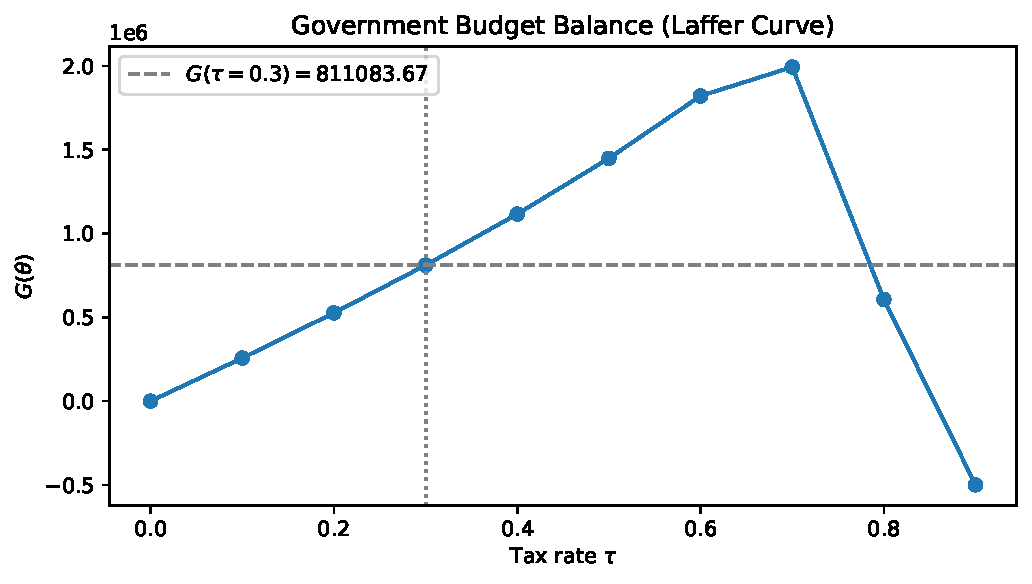
\includegraphics[width=0.6\textwidth]{../figures/q3_laffer.pdf}
  \caption{Government budget balance $G(\theta)$ as a function of the tax rate $\tau \in \{0.0, 0.1, \ldots, 0.9\}$.}
  \label{fig:q3}
\end{figure}

\paragraph{(c)} The budget balance is hump-shaped in $\tau$---a Laffer curve. At low tax rates, revenue per hour is small even though labor supply is high. As $\tau$ rises, two forces push in opposite directions: the mechanical revenue gain per unit of labor and the behavioural reduction in hours and employment. Beyond the peak, the second effect dominates: workers both reduce hours and exit employment altogether, shrinking the tax base. The expenditure side amplifies this---every worker who stops working switches from being a net contributor to a net cost, since they now collect the $\pi_0 = 0.5$ subsidy. Together, these forces cause $G(\theta)$ to turn negative at sufficiently high tax rates.
